\chapter{Camera geometry}
This chapter will introduce two important topics in camera geometry: The \emph{geometric camera model}, that describes the camera projection process, and the \emph{epipolar geometry}, that describes the geometry when seeing the same points from two different views.
Most of this chapter is based on the wonderful books by Hartley and Zisserman, and Ma et al. \cite{Hartley2004MultipleVision, Ma2004AnModels}.

\section{Geometric camera models}
In the general case, a geometric camera model is a  \emph{projection} $\pi: \bbR^3 \to \Omega$, which projects 3D points $\vecx^c \in \bbR^3$ in the camera frame $\cF_c$ onto pixels $\vecu \in \Omega$ in the image, so that
\begin{equation}
  \vecu = 
  \begin{bmatrix}
  u\\
  v
  \end{bmatrix}
  = \pi(\vecx^c).
\end{equation}
Here, $\Omega \subset \bbR^2,$ is the \emph{image domain} of all valid pixels.
The inverse of this function is the \emph{backprojection} $\pi^{-1}: \Omega \times \bbR^+ \to \bbR^3$, which maps pixels and a corresponding depth $z$ back to 3D points:
\begin{equation}
  \vecx^c =
  \begin{bmatrix}
  x^c\\
  y^c\\
  z^c
  \end{bmatrix}
  = \pi^{-1}(\vecu, z).
\end{equation}
We will in the following let $\vecu \in \bbR^2$, and assume that there is an implicit second step that ensures that $\vecu$ is a valid pixel $\in \Omega$.

When describing camera projections, it is often convenient to exploit the homogeneous point representation.
Equivalent to the homogeneous representation of 3D coordinates in Section~\ref{sec:points-coordinate-frames}, we can construct a homogeneous 2D vector from a 2D Cartesian vector with the mapping
\begin{equation} \label{eq:cart-to-homo-2d}
  \vecu = 
  \begin{bmatrix}
  u\\
  v
  \end{bmatrix}
  \in \bbR^2
  \quad \mapsto \quad
  \tilde{\vecu} = \breve{\vecu} =
  \begin{bmatrix}
  u\\
  v\\
  1
  \end{bmatrix}
  \in \bbP^2,
\end{equation}
and we can map a homogeneous vector back into a Cartesian vector with
\begin{equation} \label{eq:homo-to-cart-2d}
  \tilde{\vecu} =
  \begin{bmatrix}
  \tilde{u}\\
  \tilde{v}\\
  \tilde{w}
  \end{bmatrix}
  \in \bbP^2
  \quad \mapsto \quad
  \vecu = 
  \begin{bmatrix}
  \tilde{u} / \tilde{w}\\
  \tilde{v} / \tilde{w}
  \end{bmatrix}
  \in \bbR^2.
\end{equation}

\begin{figure}[htb]
    \centering
    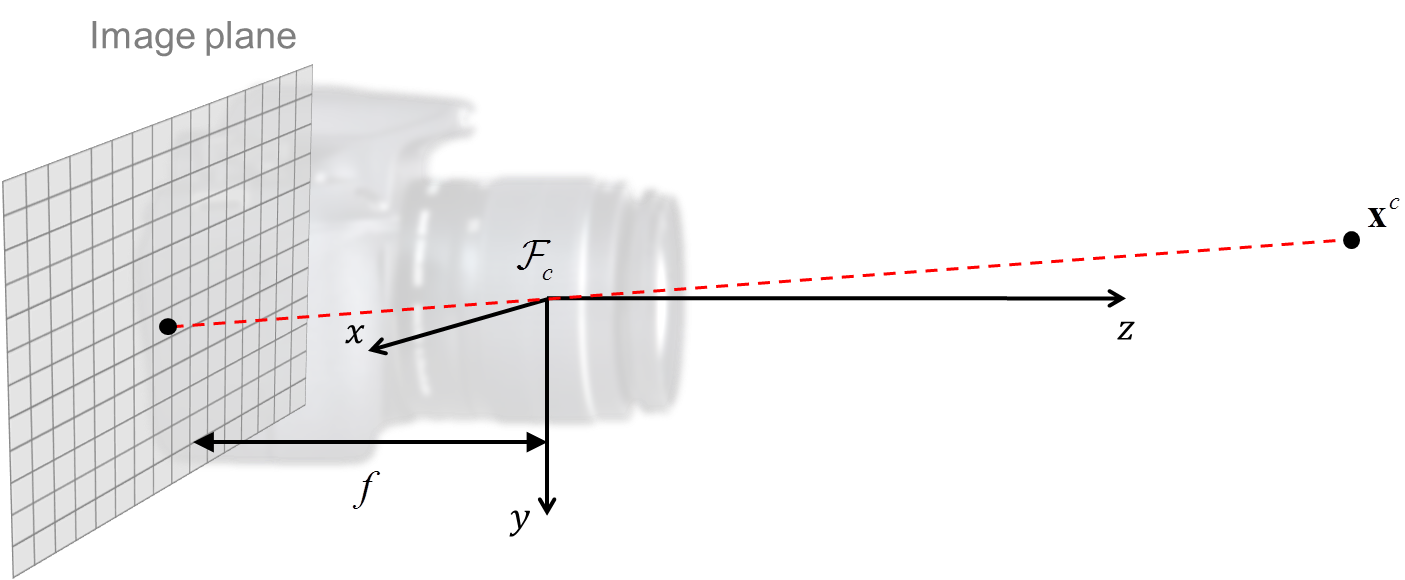
\includegraphics[height=5.5cm]{figures/perspective-camera-model-geometry.png}
    \caption{The imaging geometry in the perspective camera model.
    The camera is represented by the camera frame $\cF_c$.
    Points $\vecx^c$ in the camera frame are projected through the origin and onto the image plane at a distance $f$ behind the projective centre, where $f$ is the focal length.
    }
    \label{fig:perspective-camera-model-geometry}
\end{figure}
%
The most commonly used geometric camera model is the \emph{perspective camera model}\footnotemark.
As shown in Figure~\ref{fig:perspective-camera-model-geometry}, the camera is represented by a 3D coordinate frame $\cF_c$, with its origin at the camera's projective centre.
The $x$-axis is pointing right, the $y$-axis is pointing down, and the $z$-axis is pointing forwards along the \emph{optical axis} of the camera.
The imaging process is modelled as a central projection onto the image plane at $z = -f$, where $f$ is the \emph{focal length}.
\footnotetext{Sometimes also called the \emph{pinhole model}.}

Since the projection in Figure~\ref{fig:perspective-camera-model-geometry} results in images that are flipped upside down, it is more convenient to put the imaging plane in front of the projection centre using the \emph{frontal projection model}.
It is also convenient to define a \emph{normalised image plane} at $z = 1$, which represents an \emph{idealised camera} with focal length $1$, as illustrated in Figure~\ref{fig:perspective-camera-model_normalised}.
This lets us describe the imaging process at a fixed imaging plane, independently of the camera-specific focal length parameter $f$.

\begin{figure}[htb]
    \centering
    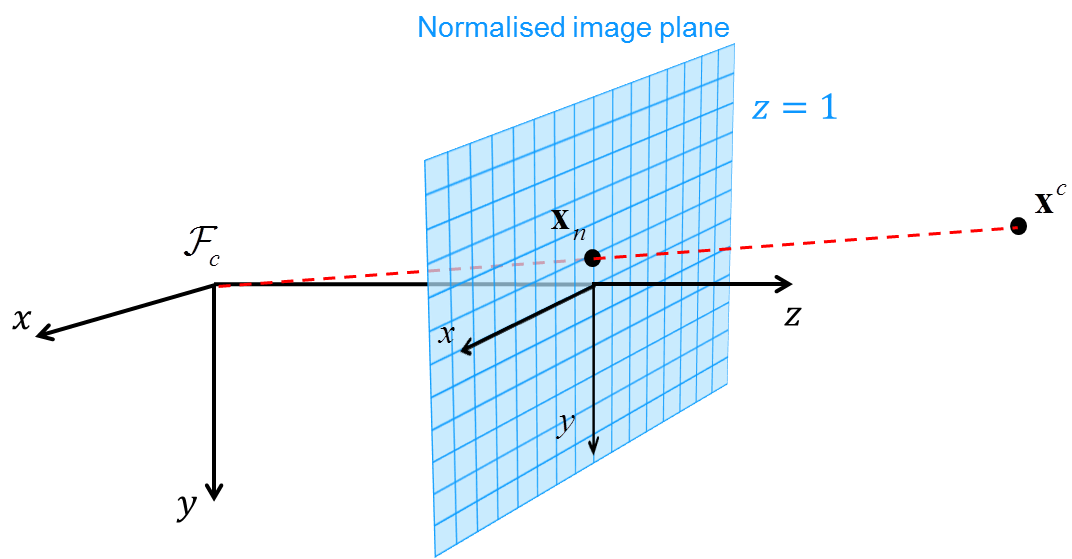
\includegraphics[height=5.5cm]{figures/perspective-camera-model_normalised.png}
    \caption{The normalised image plane is set at $z=1$ in front of the projective centre.
    This represents the perspective camera model for an idealised camera with $f = 1$.
    The point where the $z$-axis of $\cF_c$ intersects the normalised image plane is called the principal point.
    The central projection of the 3D point $\vecx^c$ onto the normalised image plane is the point $\vecx_n$, which is called the normalised image coordinate.
    }
    \label{fig:perspective-camera-model_normalised}
\end{figure}
%
We can project $\vecx^c$ onto the normalised image plane with the homogeneous \emph{perspective projection} matrix $\matPi_0$, by
\begin{equation}
  \tilde{\vecx}_n = \matPi_0 \tilde{\vecx}^c =
  \begin{bmatrix}
    1 & 0 & 0 & 0\\
    0 & 1 & 0 & 0\\
    0 & 0 & 1 & 0
  \end{bmatrix}
  \tilde{\vecx}^c = \vecx^c.
\end{equation}
On normalised form, we have that
\begin{equation} \label{eq:normalised-normalised-coordinate}
  \breve{\vecx}_n = 
  \begin{bmatrix}
    x_n\\
    y_n\\
    1
  \end{bmatrix} = 
  \begin{bmatrix}
    x^c / z^c\\
    y^c / z^c\\
    1
  \end{bmatrix}
  = \frac{1}{z^c}\vecx^c.
\end{equation}
The projected point $\tilde{\vecx}_n$ in the normalised image plane can be seen both as a Cartesian representation of the 3D point on the plane when normalised as in \eqref{eq:normalised-normalised-coordinate}, \emph{as well} as a homogeneous representation of the 2D point in the frame of the normalised image plane.
As illustrated in Figure~\ref{fig:perspective-camera-model_normalised}, this 2D frame is aligned with the $x$ and $y$ axes of the camera frame $\cF_c$, and its origin is at the \emph{principal point}, where the $z$-axis of $\cF_c$ intersects the plane.
Since $\vecx_n$ represents the image point for the idealised camera model, it is called the \emph{normalised image coordinate}, and we give it the special subscript $n$ notation.

\begin{figure}[htb]
    \centering
    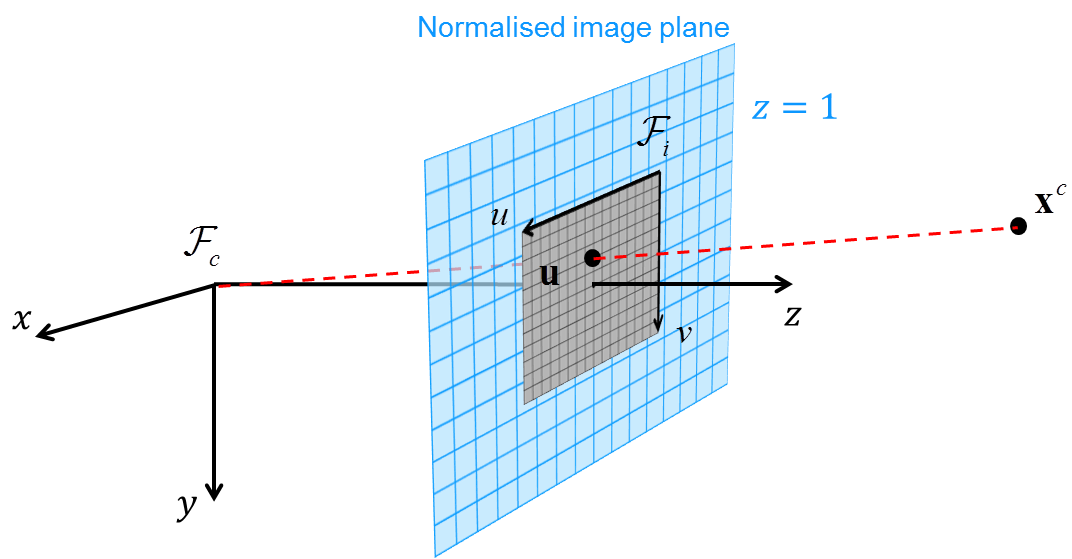
\includegraphics[height=5.5cm]{figures/perspective-camera-model.png}
    \caption{The image frame $\cF_i$, given in pixels, spans the normalised image plane.
    Its origin is at the upper-left corner of the image, its $u$-axis points right along the rows, and its $v$-axis points down along the columns.
    The mapping between normalised image coordinates and pixels is given by an affine transformation.
    }
    \label{fig:perspective-camera-model}
\end{figure}
%
As shown in Figure~\ref{fig:perspective-camera-model}, the image is represented by a 2D coordinate frame $\cF_i$ that spans the normalised image plane, with the origin at the upper-left corner of the image.
We recover the pixel coordinate $\vecu$ by mapping the normalised image coordinate $\tilde{\vecx}_n$ to the image frame $\cF_i$ with the affine transformation
\begin{equation}
  \tilde{\vecu} = \matK \tilde{\vecx}_n.
\end{equation}

The upper triangular matrix $\matK$ takes us from the idealised case to the camera-specific model.
It collects all parameters that are \emph{intrinsic} to a particular camera, and it is therefore known as the \emph{intrinsic matrix} or the \emph{calibration matrix}.
The affine transformation matrix is a combined scaling, shear and translation, and is given by
\begin{equation}
  \matK = 
  \begin{bmatrix}
    f_u & s_\theta & c_u\\
    0 & f_v & c_v\\
    0 & 0 & 1
  \end{bmatrix},
\end{equation}
where the elements of $\matK$ have the following geometric interpretation:
\begin{itemize}
  \item $f_u$ is the size of unit length in horizontal pixels.\\
  It can be expressed as $f_u = f s_u$, where $f$ is the focal length in metric units, and $s_u$ is the scaling factor that describes the horizontal pixel density in pixels per metric unit.
  \item $f_v$ is the size of unit length in vertical pixels.\\
  It can be expressed as $f_v = f s_v$, where $f$ is the focal length in metric units, and $s_v$ is the scaling factor that describes the vertical pixel density in pixels per metric unit.
  \item $c_u$ is the $u$-coordinate of the principal point in $\cF_i$.
  \item $c_v$ is the $v$-coordinate of the principal point in $\cF_i$.
  \item $s_\theta$ is the \emph{skew factor}, proportional to $\cot(\theta)$, where $\theta$ is the angle between the $u$ and $v$ axes in $\cF_i$.
\end{itemize}
Because of the structure of $\matK$, we preserve the normalised form of the homogeneous coordinates through the transformation:
\begin{equation}
  \breve{\vecu} = \matK \breve{\vecx}_n.
\end{equation}
We can estimate a calibration matrix $\matK$ by performing a camera calibration procedure such as \cite{Zhang2000ACalibration}.
It is common practice to reduce the number of parameters by dropping the skew factor.
We will therefore from here on assume that $s_\theta=0$, which will simplify the following expressions somewhat.

When $\matK$ is known, we can obtain the \emph{calibrated} normalised image coordinates from the pixel $\vecu$ by applying the inverse transformation
\begin{equation}
  \tilde{\vecx}_n = \matK^{-1} \tilde{\vecu}.
\end{equation}
The inverse transformation also preserves the normalised form:
\begin{equation} \label{eq:normalised-from-pixel}
  \breve{\vecx}_n = \matK^{-1} \breve{\vecu}.
\end{equation}

If we crop or resample images from a calibrated camera, these transformations can be encoded directly in the calibration matrix.
Since cropping corresponds to a possible translation of the principal point, and resampling corresponds to scaling, we can update the calibration matrix by applying the corresponding transformations to $\matK$.

\begin{example}[frametitle=Camera calibration matrix for downsampled images]
We calibrate a camera using $1600 \times 1200$ pixel images, and we get the following camera calibration matrix:
\begin{equation}
  \matK =
  \begin{bmatrix}
    100 &   0 & 800\\
      0 & 100 & 600\\
      0 &   0 &   1
  \end{bmatrix}.
\end{equation}
If we downscale our images with a scale factor $s = 0.5$ to $800 \times 600$ pixels, how should we modify $\matK$ in order for it to be a valid calibration matrix for the downsampled images?

Since the camera calibration matrix is an affine transformation that transforms points on the normalised image plane to pixels in the image, we can apply the scaling to $\matK$ with the homogeneous transformation matrix
\begin{equation}
    \matS_s = 
  \begin{bmatrix}
    s & 0 & 0\\
    0 & s & 0\\
    0 & 0 & 1
  \end{bmatrix}.
\end{equation}
This results in the camera calibration matrix
\begin{equation}
  \matK_{0.5} = \matS_{0.5} \matK = 
    \begin{bmatrix}
    0.5 & 0 & 0\\
    0 & 0.5 & 0\\
    0 & 0 & 1
  \end{bmatrix}
  \begin{bmatrix}
    100 &   0 & 800\\
      0 & 100 & 600\\
      0 &   0 &   1
  \end{bmatrix}
  =
  \begin{bmatrix}
    50 &   0 & 400\\
      0 & 50 & 300\\
      0 &   0 &   1
  \end{bmatrix}.
\end{equation}
\end{example}

Putting it all together, the perspective camera model on homogeneous form gives us the projection
\begin{equation}
  \tilde{\vecu} = \matK \matPi_0 \tilde{\vecx}^c = \matK \vecx^c =
  \begin{bmatrix}
    f_u & 0 & c_u\\
    0 & f_v & c_v\\
    0 & 0 & 1
  \end{bmatrix}
  \vecx^c,
\end{equation}
which first projects $\vecx^c$ onto the normalised image plane, and then applies a 2D affine transformation that maps points on the normalised image plane to pixels in the image frame $\cF_i$.
The equivalent projection function on Euclidean form is given by
\begin{equation} \label{eq:projection-function}
  \vecu = \pi_p(\vecx^c; \matK) =
  \begin{bmatrix}
    1 & 0 & 0 \\
    0 & 1 & 0 \\
  \end{bmatrix}
  \matK \frac{1}{z^c} \vecx^c =
  \renewcommand\arraystretch{2}
  \begin{bmatrix}
    f_u \dfrac{x^c}{z^c} + c_u\\
    f_v \dfrac{y^c}{z^c} + c_v \\
  \end{bmatrix}.
\end{equation}
For normalised image coordinates, we have
\begin{equation} \label{eq:normalised-projection-function}
  \vecx_n = \pi_n(\vecx^c) =
  \begin{bmatrix}
    1 & 0 & 0 \\
    0 & 1 & 0 \\
  \end{bmatrix}
  \frac{1}{z^c} \vecx^c =
  \begin{bmatrix}
    x^c / z^c\\
    y^c / z^c \\
  \end{bmatrix}.
\end{equation}

From \eqref{eq:normalised-normalised-coordinate} and \eqref{eq:normalised-from-pixel} we get the corresponding backprojection function
\begin{equation}
  \vecx^c = \pi^{-1}_p(\vecu, z; \matK) = z \matK^{-1} \breve{\vecu} = z
  \renewcommand\arraystretch{2}
  \begin{bmatrix}
    \dfrac{u - c_u}{f_u}\\
    \dfrac{v - c_v}{f_v}\\
    1
  \end{bmatrix}.
\end{equation}
For normalised image coordinates, we have
\begin{equation} \label{eq:normalised-backprojection-function}
  \vecx^c = \pi^{-1}_n(\vecx_n, z) = z \breve{\vecx}_n = z
  \begin{bmatrix}
    x_n\\
    y_n\\
    1
  \end{bmatrix}.
\end{equation}

\begin{figure}[htb]
    \centering
    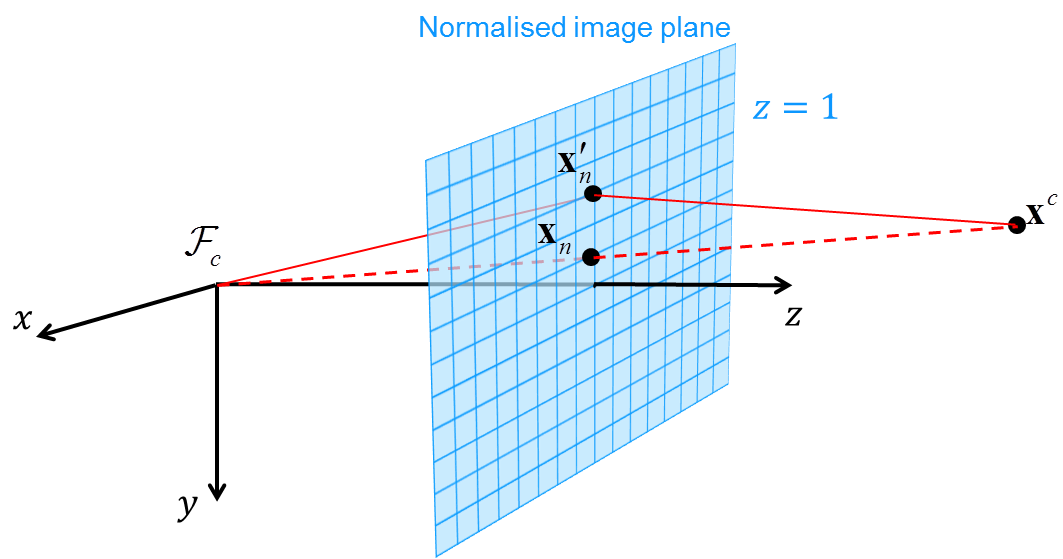
\includegraphics[height=5.5cm]{figures/radial-distortion.png}
    \caption{Typical cameras deviate from the perspective camera model geometry.
    A distortion model describes the relationship between undistorted points $\vecx_n$ and distorted points $\vecx'_n$ in the normalised image plane.
    By correcting for these deviations in the normalised image plane, the perspective camera model can still be applied in these situations.
    }
    \label{fig:radial-distortion}
\end{figure}
Practical cameras seldom fit perfectly with the perspective camera model, because they typically suffer from some kind of geometric distortion through the optical system.
This is illustrated in Figure~\ref{fig:radial-distortion}.
A \emph{distortion model} describes how a camera deviates from the perspective camera geometry, and is typically used to express the relationship between undistorted points $\vecx_n$ and distorted points $\vecx'_n$ in the normalised image plane.
A typical example is the \emph{radial distortion model}
\begin{align}
  r'{}^2 &= x'_n{}^2 + y'_n{}^2\\
  x_n &= x'_n (1 + k_1 r'{}^2 + k_2 r'{}^4)\\
  y_n &= y'_n (1 + k_1 r'{}^2 + k_2 r'{}^4),
\end{align}
where the parameters $k_1$ and $k_2$ can be estimated as part of the camera calibration process.

We will finish this discussion on geometric camera models by mentioning that there are several other models that may be more suitable than the perspective camera model in certain situations.
Examples include omnidirectional models \cite{Caruso2015Large-scaleCameras, Barreto2006UnifyingCameras} and models for underwater cameras \cite{uczynski2017TheHousings}.

\section{Epipolar geometry} \label{sec:epipolar-geometry}
\begin{figure}[htb]
    \centering
    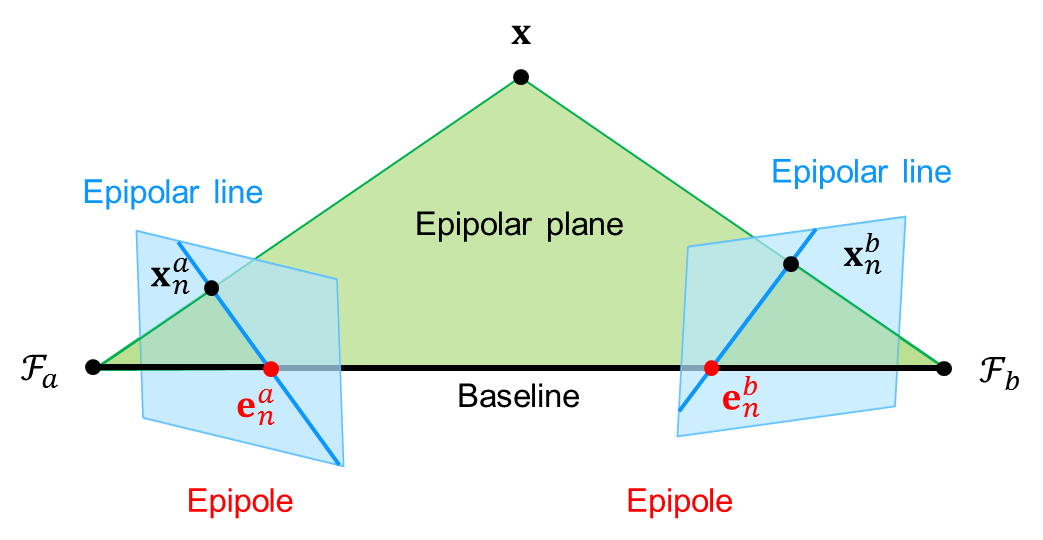
\includegraphics[width=0.75\columnwidth]{figures/epipolar-geometry.png}
    \caption{An illustration of the epipolar geometry between two perspective cameras, represented by the camera frames $\cF_a$ and $\cF_b$.
    The epipolar plane contains the point $\vecx$ and the two camera centres.
    The baseline is the line connecting the camera centres.
    The epipoles $\vece^a_n$ and $\vece^b_n$ are where the baseline intersects the image planes.
    The epipolar lines are where the epipolar plane intersects the image planes.
    Projected image points $\vecx^a_n$ and $\vecx^b_n$ corresponding to the same 3D point $\vecx$ must lie on the corresponding epipolar lines.
    This is called the epipolar constraint.
    }
    \label{fig:epipolar-geometry}
\end{figure}
Consider two perspective cameras, represented by the camera frames $\cF_a$ and $\cF_b$, as shown in Figure~\ref{fig:epipolar-geometry}.
The camera frames are related by the relative pose
\begin{equation} \label{eq:epipolar-pose-ab}
  \matT_{ab} =
  \begin{bmatrix}
    \matR_{ab} & \vect^a_{ab}\\
    \matr{0} & 1
  \end{bmatrix},
\end{equation}
or, equivalently, the inverse pose
\begin{equation}
  \matT_{ba} = \matT_{ab}^{-1} =
  \begin{bmatrix}
    \matR_{ba} & \vect^b_{ba}\\
    \matr{0} & 1
  \end{bmatrix}.
\end{equation}
Observing the same point $\vecx$ with these two cameras puts a strong geometric constraint on the point correspondence in the two images.
This constraint is called the \emph{epipolar constraint}.

Figure~\ref{fig:epipolar-geometry} shows the \emph{epipolar plane}, which is the plane containing the point $\vecx$ and the two camera centres of $\cF_a$ and $\cF_b$.
The line joining the camera centres is the \emph{baseline}, and the \emph{epipoles} are where the baseline intersects the image planes.
This means that the epipoles are the images of the other camera centre.
In normalised image coordinates, they are given by
\begin{align}
  \tilde{\vece}^a_n &= \vect^a_{ab}\\
  \tilde{\vece}^b_n &= \vect^b_{ba}.
\end{align}
Given the camera calibration matrices $\matK_a$ and $\matK_b$, the corresponding pixel points in the images are given by
\begin{align}
  \tilde{\vece}^a &= \matK_a \vect^a_{ab}\\
  \tilde{\vece}^b &= \matK_b \vect^b_{ba}.
\end{align}

\begin{figure}[htb]
    \centering
    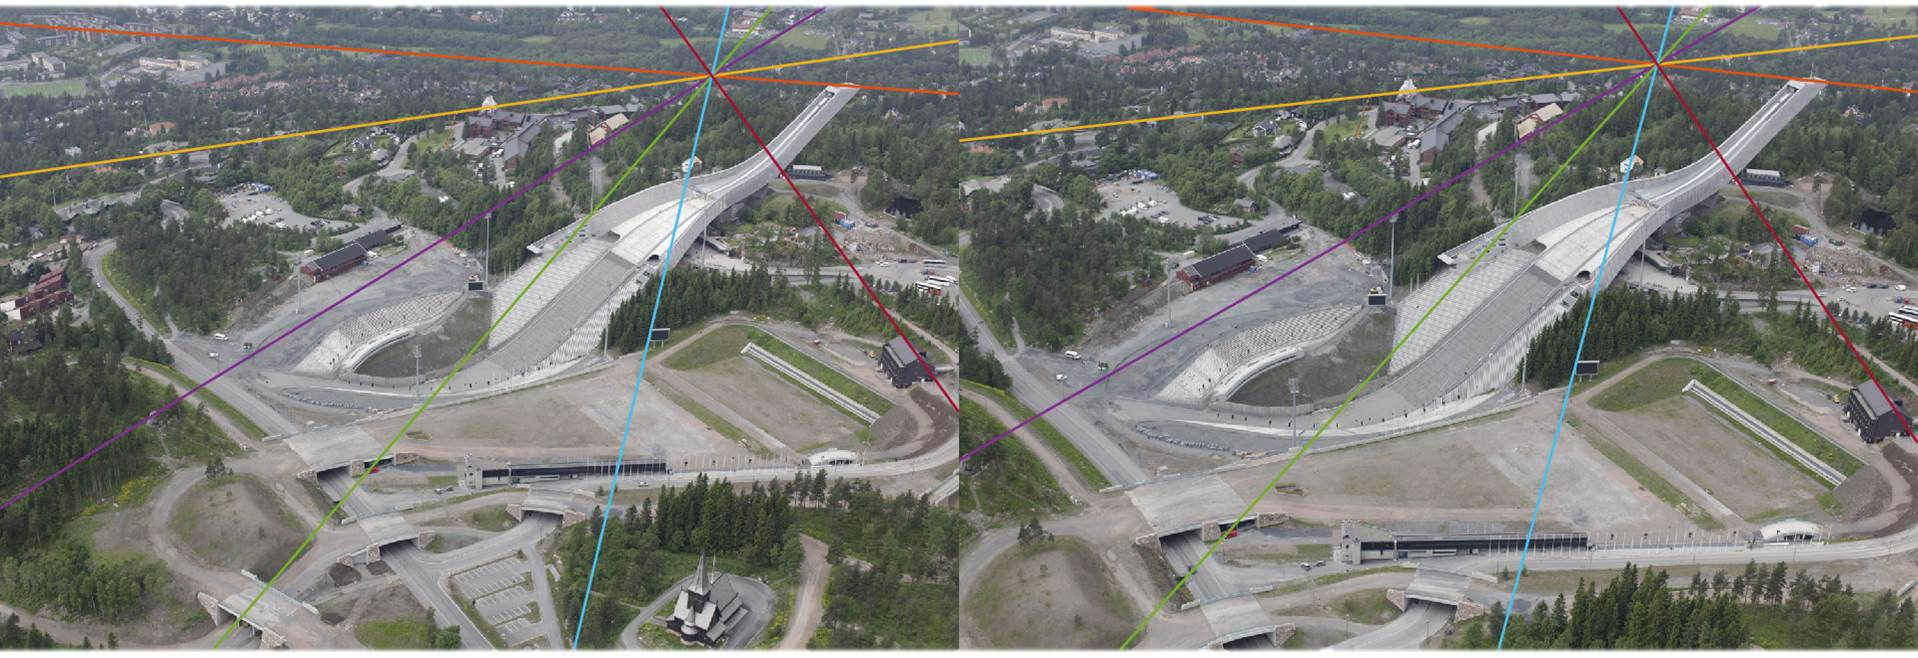
\includegraphics[width=\columnwidth]{figures/epipoles-example.jpg}
    \caption{An example of epipolar lines between two images that was captured sequentially while moving towards the Holmenkollen ski jump.
    In the left image, we see the epipolar lines intersect at the epipole, corresponding to the image of the camera centre in the second position (when the right image was captured).
    In the right image, we see the epipole corresponding to the the first camera position, projected in from behind.
    Corresponding epipolar lines are given the same colour.
    Notice that objects in the scene lie on corresponding epipolar lines, in accordance with the epipolar constraint.
    }
    \label{fig:epipoles-example}
\end{figure}
The lines where the epipolar plane intersects the image planes is called the \emph{epipolar lines}.
Informally, the epipolar constraint says that corresponding points in the two images \emph{must} lie on corresponding epipolar lines, since the cameras and the associated 3D point form a common epipolar plane.
Figure~\ref{fig:epipoles-example} shows a few examples of corresponding epipolar lines in two different images.


\begin{figure}[htb]
    \centering
    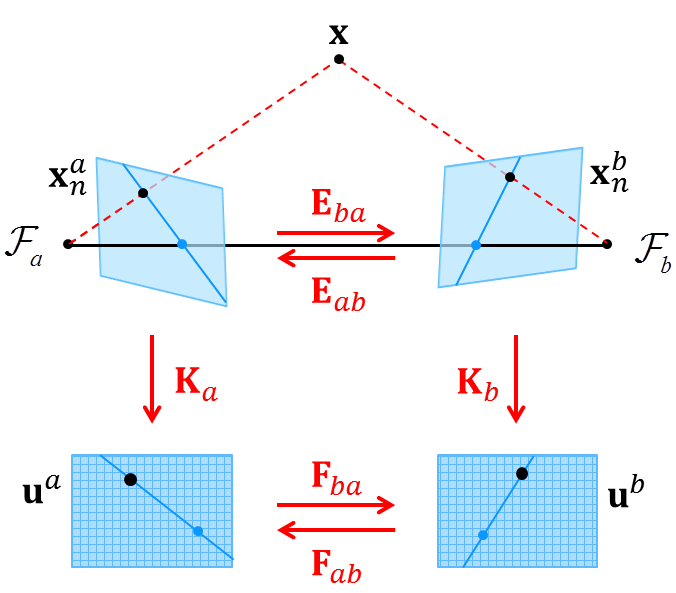
\includegraphics[width=0.5\columnwidth]{figures/essential-and-fundamental-matrices.png}
    \caption{The essential matrices $\matE_{ab}$ and $\matE_{ba}$ represent the epipolar constraint in the normalised image planes.
    The fundamental matrices $\matF_{ab}$ and $\matF_{ba}$ represent the same epipolar constraint in the images.
    They can be computed from the essential matrices via the camera calibration matrices $\matK_a$ and $\matK_b$.
    }
    \label{fig:essential-and-fundamental-matrices}
\end{figure}
The epipolar constraint can be represented mathematically by the \emph{essential matrix} $\matE \in \bbR^{3 \times 3}$ in the normalised image plane, and by the \emph{fundamental matrix} $\matF \in \bbR^{3 \times 3}$ in the image.
A correspondence $\vecx^a_n \leftrightarrow \vecx^b_n$ in the normalised image planes of the two cameras $\cF_a$ and $\cF_b$ must satisfy the equation
\begin{equation} \label{eq:essential-epipolar-constraint}
  \tilde{\vecx}^a_n{}\trans \matE_{ab} \tilde{\vecx}^b_n = 0.
\end{equation}
The essential matrix $\matE_{ab}$ is given by
\begin{equation} \label{eq:essential-structure}
  \matE_{ab} = \skewsymm{\vect^a_{ab}} \matR_{ab},
\end{equation}
which is related to the pose $\matT_{ab}$ in \eqref{eq:epipolar-pose-ab}.
The equation
\begin{equation}
  \tilde{\vecx}^b_n{}\trans \matE_{ba} \tilde{\vecx}^a_n = 0,
\end{equation}
with the essential matrix
\begin{equation}
  \matE_{ba} = \matE_{ab}\trans = \skewsymm{\vect^b_{ba}} \matR_{ba},
\end{equation}
is an equivalent representation of the constraint in \eqref{eq:essential-epipolar-constraint}.

As illustrated in Figure~\ref{fig:essential-and-fundamental-matrices}, the epipolar constraint extends naturally to pixel correspondences $\tilde{\vecu}^a \leftrightarrow \tilde{\vecu^b}$ via the camera calibration matrices $\matK_a$ and $\matK_b$.
The pixel correspondences must satisfy the equation
\begin{equation} \label{eq:fundamental-epipolar-constraint}
  \tilde{\vecu}^a{}\trans \matF_{ab} \tilde{\vecu}^b = 0,
\end{equation}
where the fundamental matrix $\matF_{ab}$ is given by
\begin{equation}
  \matF_{ab} = \matK_a\invtrans \matE_{ab} \matK_b^{-1}.
\end{equation}
The equivalent fundamental matrix $\matF_{ba}$ is similarly given by
\begin{equation}
    \matF_{ba} = \matF_{ab}\trans = \matK_b\invtrans \matE_{ba} \matK_a^{-1}.
\end{equation}

\begin{figure}[htb]
    \centering
    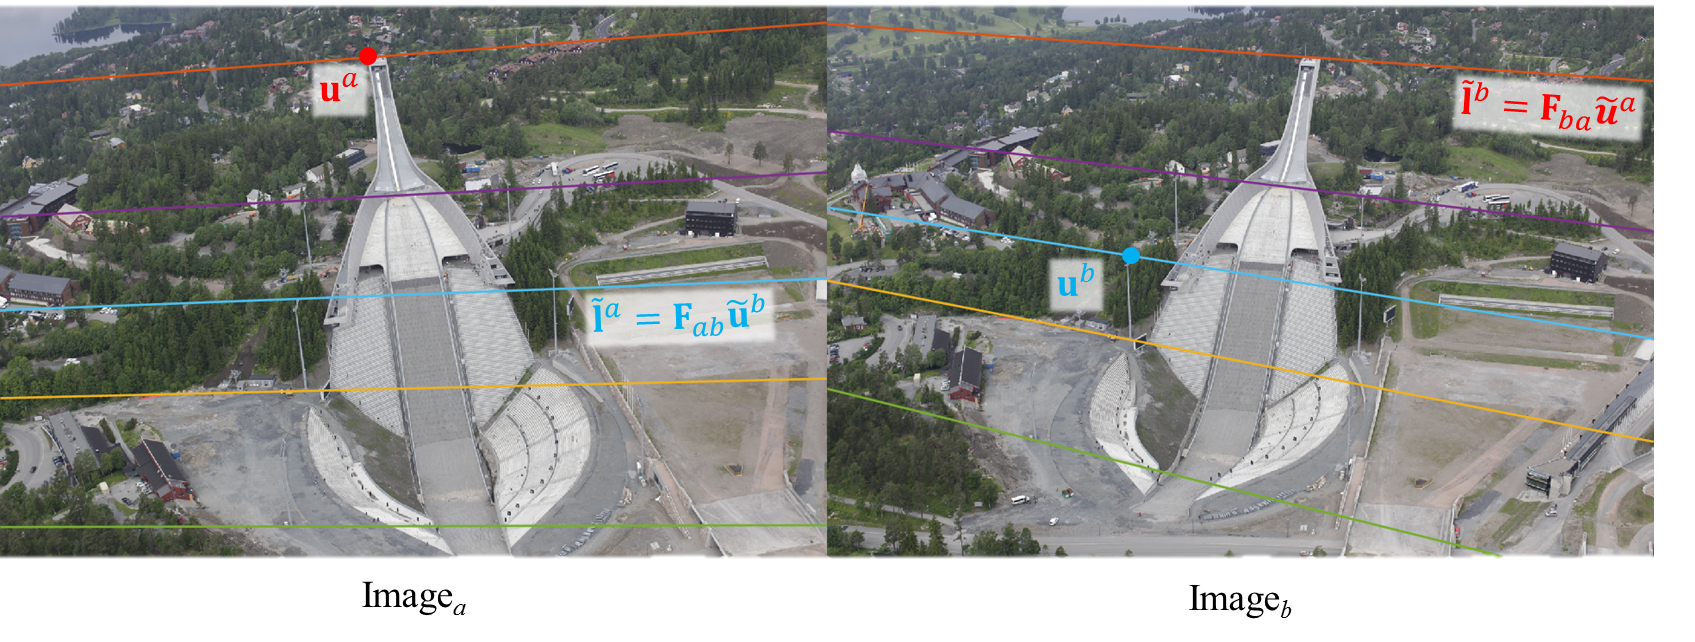
\includegraphics[width=\columnwidth]{figures/epipolar-lines-example.png}
    \caption{An example of computing epipolar lines in one image, given a point in the other image and the fundamental matrix.
    Corresponding epipolar lines are given the same colour.
    Notice that objects in the scene lie on corresponding epipolar lines in the images.
    }
    \label{fig:epipolar-lines-example}
\end{figure}
Since
\begin{equation}
  \tilde{\vecx}\trans \tilde{\vecl} = 0, \qquad \tilde{\vecl} =
  \begin{bmatrix}
    a\\
    b\\
    c
  \end{bmatrix}
  \in \bbP^2
\end{equation}
is the homogeneous representation of the line
\begin{equation}
  ax + by + c = 0,
\end{equation}
we see from \eqref{eq:essential-epipolar-constraint} that
\begin{equation}
  \tilde{\vecl}^a_n = \matE_{ab} \tilde{\vecx}^b_n
\end{equation}
is the epipolar line in the normalised image plane of $\cF_a$ corresponding to the point $\tilde{\vecx}^b_n$ in $\cF_b$.
Equivalently, we see from \eqref{eq:fundamental-epipolar-constraint} that
\begin{equation}
  \tilde{\vecl}^a = \matF_{ab} \tilde{\vecu}^b
\end{equation}
is the corresponding epipolar line in the image of $\cF_a$.
As illustrated in Figure~\ref{fig:epipolar-lines-example}, we can find the corresponding epipolar lines in $\cF_b$ by using $\matE_{ba}$ and $\matF_{ba}$.

We can restrict the search for correspondences by traversing along the epipolar line.
Given a set of putative point correspondences, we can test their validity by computing the distances to their corresponding epipolar lines.
The distance $d(\tilde{\vecu}, \tilde{\vecl})$ between a homogeneous point $\tilde{\vecu}$ and a homogeneous line $\tilde{\vecl}$ is given by
\begin{equation}
  d(\tilde{\vecu}, \tilde{\vecl}) = \frac{\tilde{\vecu}\trans \tilde{\vecl}}{\sqrt{\tilde{l}_1 + \tilde{l}_2}}.
\end{equation}
Although it is a necessary requirement that $d(\tilde{\vecu}^a, \matF_{ab} \tilde{\vecu}^b)$ is small for $\tilde{\vecu}^a$ and $\tilde{\vecu}^b$ to be a valid point correspondence, it important to emphasise that this is not sufficient to guarantee its validity.
It only suggests that the two points lie in the same epipolar plane.

We can estimate the fundamental matrix $\matF$ from point correspondences using the 7- or 8-point algorithms \cite{Hartley2004MultipleVision}.
The essential matrix $\matE$ can be estimated from point correspondences with the 5-point algorithm \cite{Nister2004AnProblem}.
We can also compute the essential matrix from the fundamental matrix by
\begin{align}
  \matE_{ab} = \matK_a\trans \matF_{ab} \matK_b.
\end{align}
We will see in Chapter~\ref{ch:estimating-pose-and-structure} that the structure of the essential matrix \eqref{eq:essential-structure} can be exploited to estimate the relative pose between images up to scale.

\begin{figure}[htb]
    \centering
    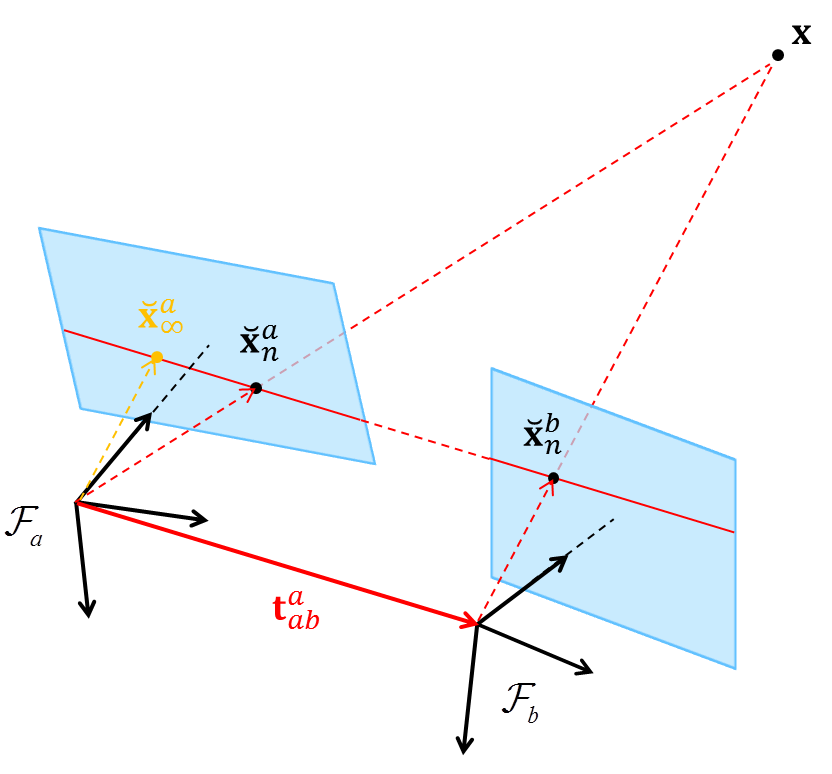
\includegraphics[width=0.6\columnwidth]{figures/epipolar-known-pose.png}
    \caption{When we know the pose of $\cF_b$ relative to $\cF_a$, we can map the image point $\breve{\vecx}^b_n$ into $\cF_a$ by $\tilde{\vecx}^a_{\infty} = \matR_{ab} \breve{\vecx}^b$.
    This corresponds to the image of $\vecx$ when $\vecx$ is infinitely far away.
    The point $\breve{\vecx}^a_n$ will in this example lie on the epipolar line to the right of $\tilde{\vecx}^a_{\infty}$ (in the direction of $\vect^a_{ab}$) for all other depths, restricting the search for valid correspondences further.
    }
    \label{fig:epipolar-known-pose}
\end{figure}
When the relative pose between the cameras are known, we can also express the epipolar line as a function of depth from the other camera.
This can for $\cF_a$ be expressed as as
\begin{equation} \label{eq:epipolar-line-known-pose-normalised}
  \tilde{\vecx}^a_n = \matR_{ab} \breve{\vecx}^b_n + \frac{1}{z^b} \vect^a_{ab},
\end{equation}
where $\breve{\vecx}^b_n$ is the normalised point correspondence in the normalised image plane of $\cF_b$ and $z^b$ is the depth from $\cF_b$.
Since we can think of $\breve{\vecx}^b_n$ as a 3D vector on the normalised image plane of $\cF_b$, the first term in \eqref{eq:epipolar-line-known-pose-normalised} rotates $\breve{\vecx}^b_n$ into the frame $\cF_a$ of the other camera (Figure~\ref{fig:epipolar-known-pose}).
These lines of sight are parallel, and correspond to the projections of a 3D point without observable depth.
This is because the motion between the cameras were without translation, or because the 3D point is ``infinitely'' far away.
We therefore write this projection as
\begin{equation}
  \tilde{\vecx}^a_{\infty} = \matR_{ab} \breve{\vecx}^b_n.
\end{equation}

The second term in \eqref{eq:epipolar-line-known-pose-normalised} moves $\tilde{\vecx}^a_n$ along the epipolar line defined by $\tilde{\vecx}^a_{\infty}$ and the epipole $\vect^a_{ab}$.
By increasing the \emph{inverse depth} $1/z^b$, we move away from $\tilde{\vecx}^a_{\infty}$, faster and faster as the depth decreases.

\begin{figure}[htb]
    \centering
    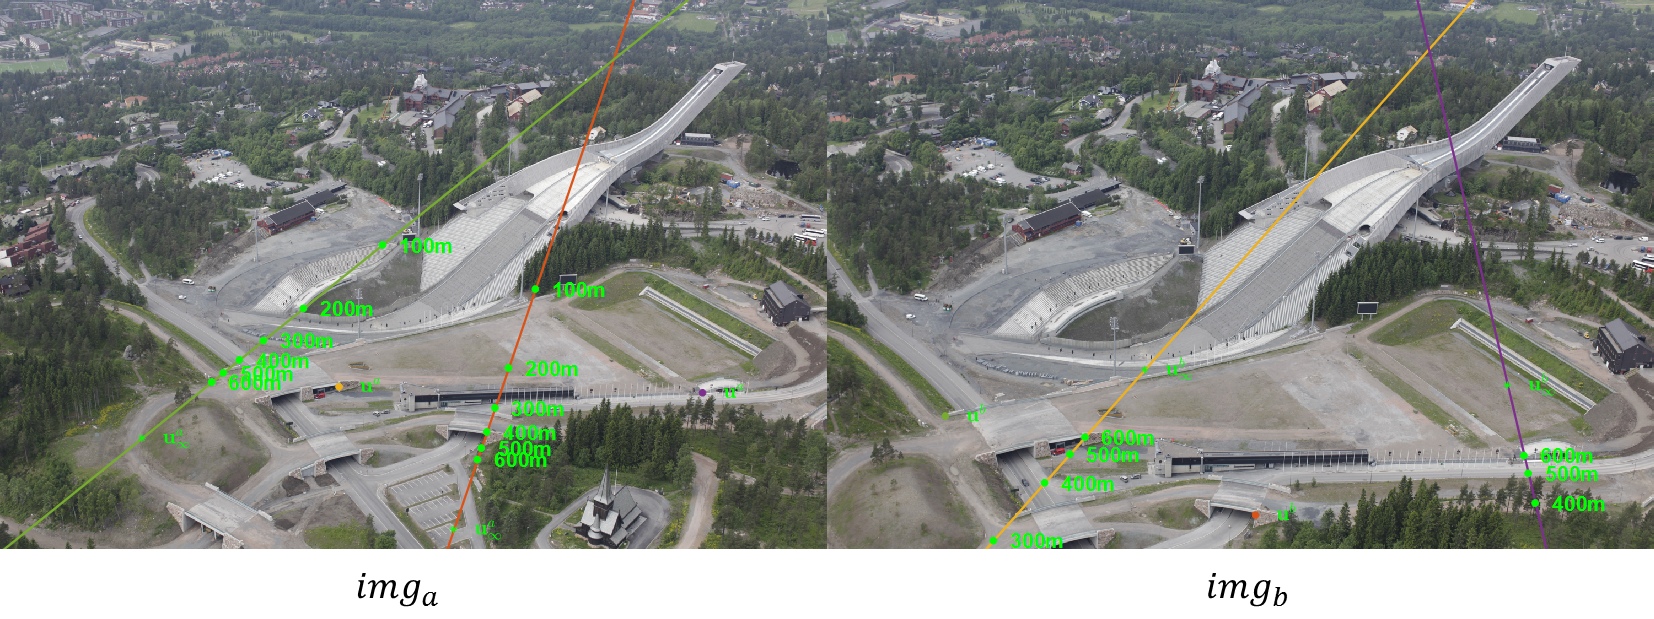
\includegraphics[width=\columnwidth]{figures/epipolar-range-example.png}
    \caption{Epipolar lines with depth.
    This example shows two chosen points in each image, with the corresponding epipolar lines in the other image given the same colour.
    The corresponding depth for the chosen points along the epipolar lines according to \eqref{eq:epipolar-line-known-pose-image} are shown, together with the limit at $\vecu_\infty$. 
    }
    \label{fig:epipolar-range-example}
\end{figure}
The corresponding representation of the epipolar line in the image is given by
\begin{equation} \label{eq:epipolar-line-known-pose-image}
\tilde{\vecu}^{a} = \tilde{\vecu}^a_{\infty} + \frac{1}{z^b}\matK_{a} \vect^a_{ab},
\end{equation}
with
\begin{equation}
  \tilde{\vecu}^a_{\infty} = \matK_a \matR_{ab} \matK^{-1}_b \breve{\vecu}^b
\end{equation}
The distance between the pixels 
\begin{equation}
  d = \norm{\vecu^a - \vecu^a_\infty}
\end{equation}
is called the \emph{disparity}, and is a measure of the observed parallax between the cameras.

\begin{example}[frametitle=Stereo geometry]
{
  \centering
  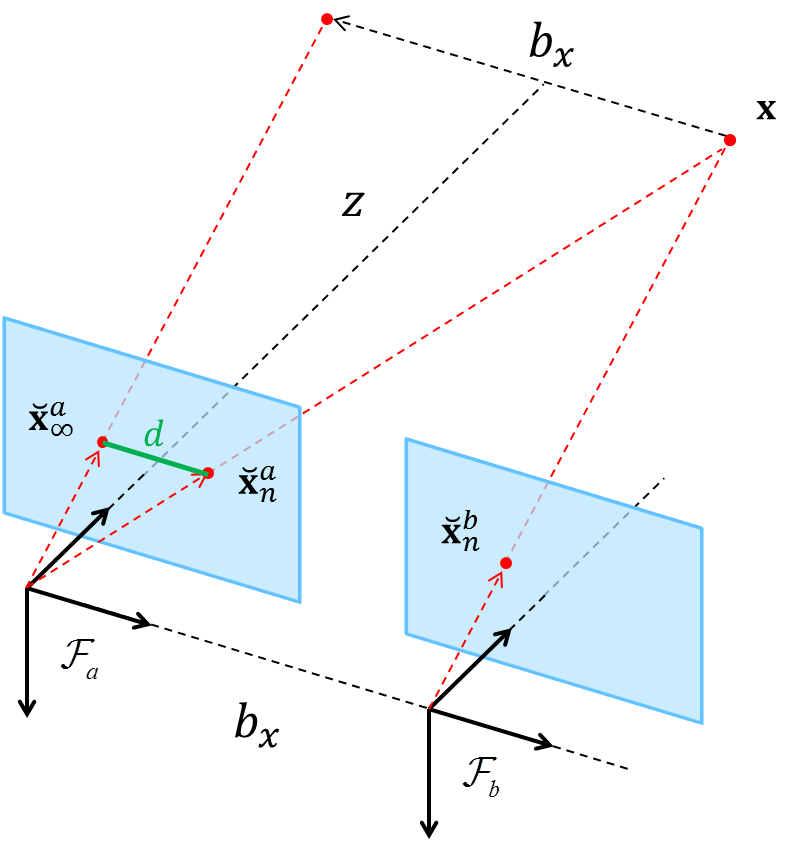
\includegraphics[width=0.6\columnwidth]{figures/stereo-geometry.png}
  \captionsetup{type=figure}
  \captionof{figure}{The ideal stereo geometry.
    The cameras have identical orientation, and baseline along the $x$-axis with distance $b_x$.}
  \label{fig:stereo-geometry}
  \par
}
Stereo imaging exploits a special case of the epipolar geometry presented in this section.
In stereo geometry
\begin{equation}
  \matK_a = \matK_b = \matK,
\end{equation}
\begin{equation}
  \matR_{ab} = \matR_{ba} = \matI, 
\end{equation}
and the translation between the cameras are typically along the $x$-axis
\begin{equation}
  \vect^a_{ab} = 
  \begin{bmatrix}
    b_x\\
    0\\
    0
  \end{bmatrix},
\end{equation}
where $b_x$ is the length of the baseline.
This means that the epipoles are at the infinity, 
\begin{equation}
  \breve{\vecu}^a_{\infty} = \breve{\vecu}^b,
\end{equation}
and the epipolar lines are horizontal along the rows in the images:
\begin{equation}
  \breve{\vecu}^{a} = \breve{\vecu}^b + 
  \renewcommand\arraystretch{1.5}
  \begin{bmatrix}
    f_u\dfrac{b_x}{z}\\
    0\\
    0
  \end{bmatrix}.
\end{equation}
The disparity is therefore given as
\begin{equation}
  d = \norm{\vecu^a - \vecu^a_\infty} = u^a - u^b = f_u\dfrac{b_x}{z}.
\end{equation}
This results in a simple expression for the depth given the disparity $d = u^a - u^b$:
\begin{equation}
  z = f_u\dfrac{b_x}{d}.
\end{equation}
\end{example}

We can use this representation of the epipolar lines to restrict the search for correspondences between images even further.
Clearly, the relevant part of the epipolar line can always be restricted on one end by $\tilde{\vecu}^a_{\infty}$ (or $\tilde{\vecx}^a_{\infty}$ on the normalised image plane), if it is visible in the image.
With information about the relevant interval of the depth $z^b$, we can use \eqref{eq:epipolar-line-known-pose-normalised} and \eqref{eq:epipolar-line-known-pose-image} to define the corresponding relevant segment on the epipolar line.
We will see in Chapter~\ref{ch:estimating-pose-and-structure} that this representation can also be used to estimate the depth to a point, given the relative pose and point correspondence.

